\documentclass[11pt, oneside]{article}   	% use "amsart" instead of "article" for AMSLaTeX format
\usepackage{geometry}                		% See geometry.pdf to learn the layout options. There are lots.
\geometry{letterpaper}                   		% ... or a4paper or a5paper or ... 
%\geometry{landscape}                		% Activate for for rotated page geometry
%\usepackage[parfill]{parskip}    		% Activate to begin paragraphs with an empty line rather than an indent
\usepackage{graphicx}				% Use pdf, png, jpg, or eps� with pdflatex; use eps in DVI mode
								% TeX will automatically convert eps --> pdf in pdflatex		
\usepackage{amssymb}

\title{Liste}
%\author{Fabrizio Demaria}
\date{}							% Activate to display a given date or no date

\begin{document}
\maketitle
%%%%%%%%%%%%%%%%%%%%%%%%%%%%%%%%%%%%%%%%%%%%%%%%%%%%%%%%%%%%%%%%%%%%%%%%%%%%%%

\section{Richiami logici sulle liste}

Le liste sono strutture sequenziali in cui un insieme di dati si riferisce mutualmente tramite puntatori (referimenti).
Tra le principali strutture a lista ricordiamo le successive.

La Figura~\ref{fig:lista} rappresenta una lista semplice con un unico puntatore.

\begin{figure}[h]
\begin{center}
\label{fig:lista}
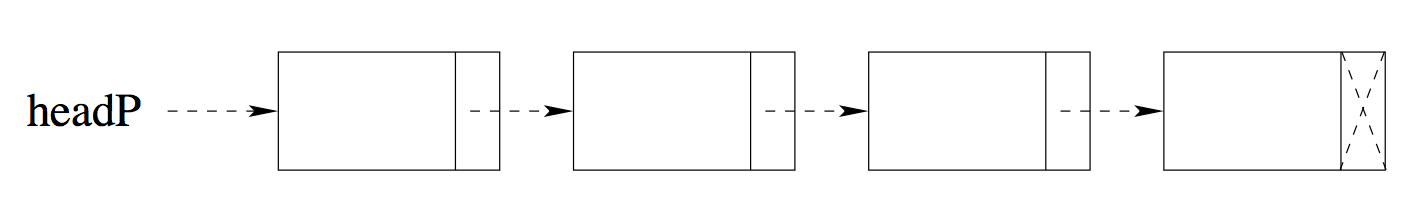
\includegraphics[angle=0,width=0.8\textwidth]{listasemplice}
\end{center}
\caption{Esempio di lista semplice mono-direzionale.}
\end{figure}

La sequenzialit\`a della struttura \`e rappresentata dalla necessit\`a di utilizzare i puntatori per la relativa visita. Tra le liste di maggiore utilizzo ricordiamo:

\begin{itemize}
\item
le strutture a pila (o stack).
Sono strutture nelle quali la strategia di inserzione e estrazione
avviene secondo lo schema LIFO ovveo Last In First Out.
\item
le code (o queue).
Sono strutture nelle quali la strategia di inserzione e estrazione
avviene secondo lo schema FIFO ovveo First In First Out.
\item
le strutture ordinate.
Sono strutture nelle quali la strategia di inserzione e estrazione
avviene utilizzando un certo ordinamento (normalmente numerico o
lessicografico) delle chiavi.
\end{itemize}

%Errore con l'uso di ref{fig:------}... Il numero di riferimento esce sbagliato!
La Figura~\ref{fig:listaDoppia} rappresenta una lista con doppio puntatore, ovvero percorribile in entrambi i sensi.

\begin{figure}[h]
\begin{center}
\label{fig:listaDoppia}
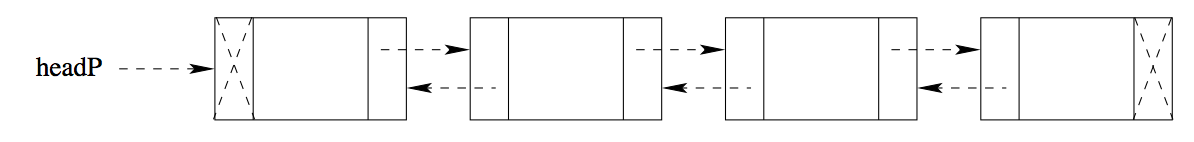
\includegraphics[angle=0,width=0.8\textwidth]{listadoppia}
\end{center}
\caption{Esempio di lista doppia bi-direzionale.}
\end{figure}

Essa risulta ancora una struttura di tipo sequenziale, ma la scansione pu\`o essere effettuata in entrambe le direzioni (da destra a sinistra oppure da sinistra a destra).

La Figura~\ref{fig:listaListe} rappresenta una lista di liste, ovvero un lista principale a cui, per ogni elemento \`e associata una lista secondaria.

\begin{figure}[h]
\begin{center}
\label{fig:listaListe}
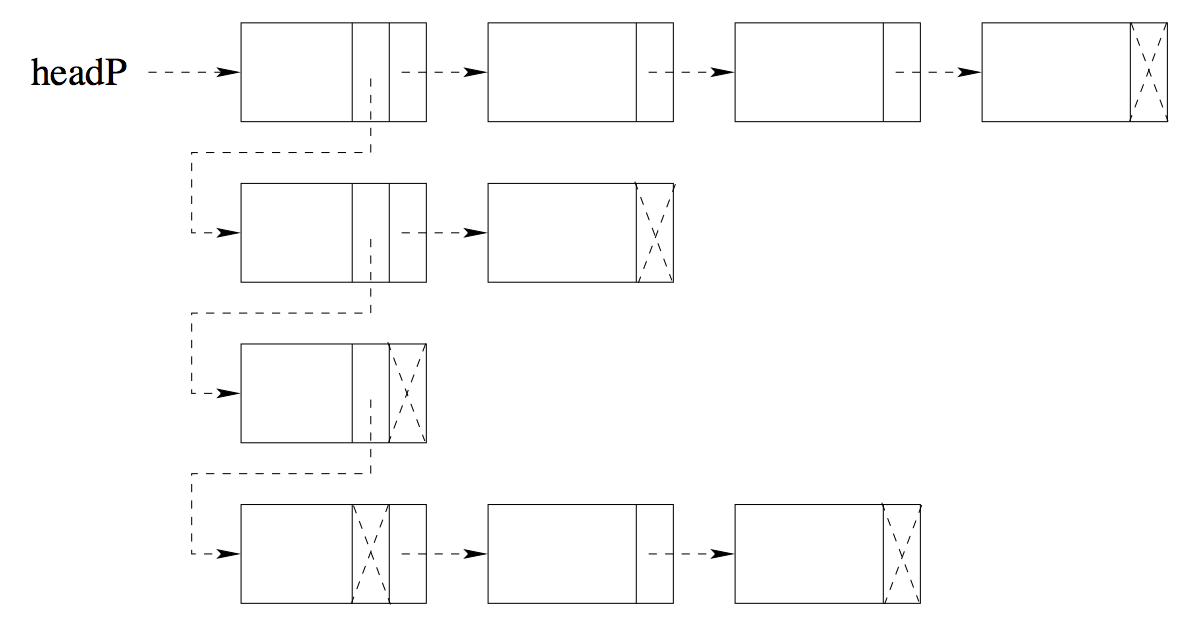
\includegraphics[angle=0,width=0.8\textwidth]{listaliste}
\end{center}
\caption{Esempio di lista di liste.}
\end{figure}

L'ultima struttura presentata permette sostanzialmente una generalizzazione delle matrici bidimensionali e viene in genere utilizzata per la memorizzazione di dati raggruppati in sottoinsiemi (tipico esempio \`e quello di un insieme di fornitori, memorizzati lungo la lista principale verticale, ad ognuno dei quali \`e associato un insieme di prodotti, la relativa lista orizzontale).
\\

Le {\em liste concatenate} sono dunque insiemi di elementi che non vengono memorizzati consecutivamente in memoria, ma registrati come nodi accessibili per mezzo di puntatori (riferimenti). Le liste permettono una gestione approfondita della memoria, in quanto i vari nodi possono essere allocati e rilasciati a seconda delle necessit\`a durante l'esecuzione di un programma (runtime): le liste sono un esempio di {\em struttura dati dinamica}. 

Tuttavia, questo sistema non permette l'{\em accesso diretto} ad un nodo specifico: nel caso delle liste si parla di {\em accesso sequenziale}, che prevede l'attraversamento della lista da uno dei suoi estremi (per i quali il puntatore deve essere disponibile) per il raggiungimento di un nodo specifico. Il tempo di accesso dipender\`a dalla posizione del nodo nella lista, e il costo dell'operazione \`e dunque lineare: $O(n)$.
\\

Nel linguaggio di programmazione C le liste possono essere implementate adottando {\em struct} (che rappresentano i nodi della struttura) connesse mediante puntatori. Tra i valori della struct \`e presente il valore chiave {\em k} con il quale \`e possibile identificare i vari nodi. In questo caso, il risultato di una operazione SEARCH \`e il puntatore al nodo desiderato (se questo \`e presente nella lista). 


\subsection{Stack}
Uno stack pu\`o essere implementato mediante una lista concatenata. In un stack, l'operazione di INSERT \`e chiamata PUSH, mentre l'operazione DELETE \`e chiamata POP. La procedura di inserimento e cancellazione di elementi in uno stack segue la strategia denominata LIFO (Last In First Out): PUSH inserisce un elemento in cima allo stack e l'operazione POP legge ed elimina l'elemento in cima allo stack (l'ultimo elemento inserito).

\begin{figure}[h]
\begin{center}
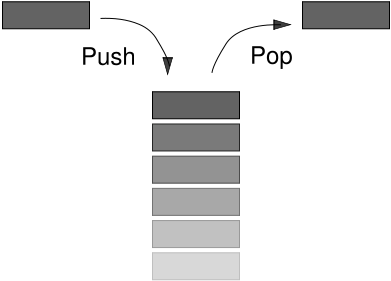
\includegraphics[angle=0,width=0.4\textwidth]{stack}
\end{center}
\caption{Operazioni PUSH e POP per uno stack}
\end{figure}

Se si tenta di estrarre un elemento (POP) da uno stack vuoto, si ha un {\bf underflow} dello stack. L'uso di liste permette di poter aggiungere un numero virtualmente infinito di elementi, ma si usasse un array di dimensione fissa per implementare lo stack si potrebbe arrivare ad una situazione chiamata {\bf overflow} se si cercasse di inserire un elemento in uno stack pieno.

Sia l'operazione di PUSH che l'operazione di POP operano sullo stesso estremo della lista e necessitano solamente del puntatore all'elemento in cima allo stack (detto {\em head}).

\subsection{Coda}
Una lista concatenata pu\`o essere usata per implementare una coda. L'operazione INSERT per una coda \`e chiamata ENQUEUE, mentre l'operazione DELETE \`e chiamata DEQUEUE. La coda \`e una struttura dati che prevede una strategia FIFO (First In First Out). A differenza dello stack, un elemento inserito nella coda tramite ENQUEUE viene posizionato in fondo alla coda, mentre l'operazione DEQUEUE estrae sempre l'elemento all'inizio della coda (l'elemento inserito per primo tra quelli nella coda).


\begin{figure}[h]
\begin{center}
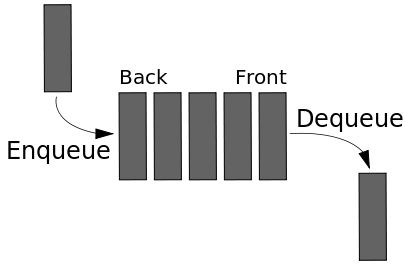
\includegraphics[angle=0,width=0.4\textwidth]{queue}
\end{center}
\caption{Operazioni di ENQUEUE e DEQUEUE per una coda}
\end{figure}

Anche per la coda sono validi i concetti di overflow e underflow, simili a quelli descritti per lo stack.

Per gestire le operazioni su una coda si possono adottare due approcci differenti. Considerando che le operazioni di DEQUEUE e ENQUEUE operano sui due estremi opposti della lista, si pu\`o pensare di mantenere disponibili i rispettivi puntatori {\em head} e {\em tail}. \`E anche possibile usare il solo puntatore {\em tail} e far si che l'elemento in fondo alla coda punti all'elemento in cima alla coda.

\subsection{Liste ordinate}

Una lista ordinata \`e una lista {\em generica} caratterizzata da un ordinamento lineare che corrisponde all'ordine delle chiavi memorizzate nei vari elementi della lista stessa. \`E dunque possibile elaborare una procedura di inserimento che mantenga la lista ordinata. 

Sebbene la ricerca di un elemento nella lista ordinata rimanga un'operazione ad accesso sequenziale, \`e possibile fermare la ricerca non appena sia stata raggiunta una chiave con valore maggiore rispetto a quella desiderata (proseguire la ricerca con valori maggiori \`e inutile): questo approccio permette di ottimizzare la procedura di SEARCH nel caso in cui l'oggetto della ricerca non sia presente nella lista.

\end{document}  






\begin{figure}[h]
\begin{center}
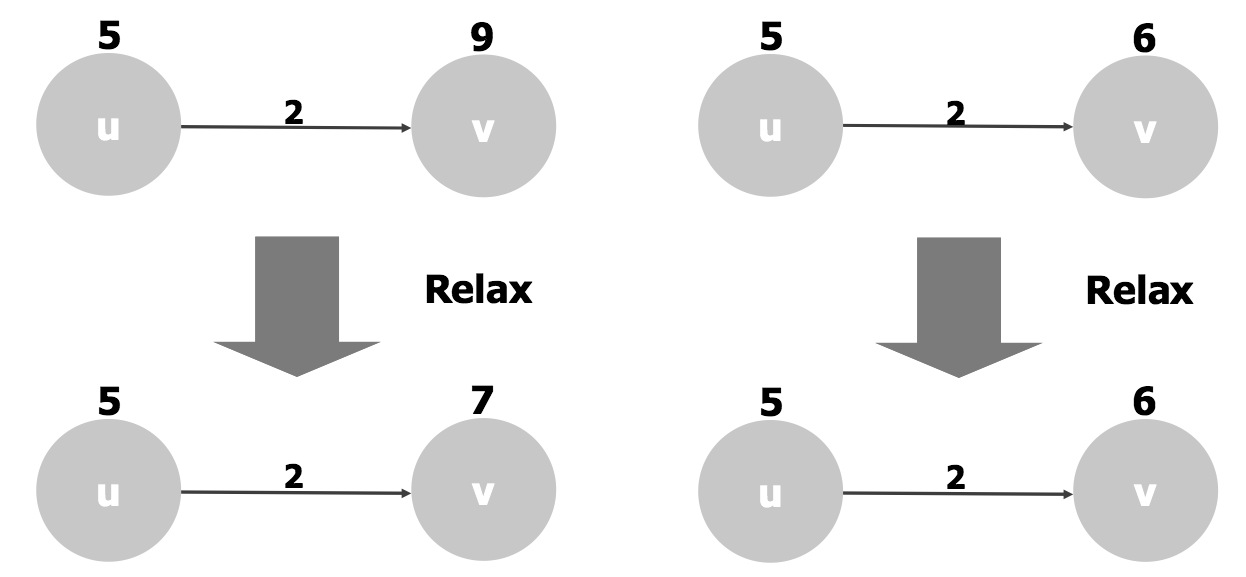
\includegraphics[angle=0,width=0.8\textwidth]{relax}
\end{center}
\caption{Due esempi di rilassamento di un arco $(u,v)$}
\end{figure}